\chapter{Conclusion}

This chapters summarizes the results of this thesis

\subsection{Churn prediction}

We summarize in this section the main results of the experiments on churn
prediction. The numerical results are reproduced in table
\ref{tab:results_conclusion}. We observe that feature selection does not reduce
performance if at least 30 of the most important variables are selected. Also,
adding difference and ratio variables reduces the performance if no feature
selection is conducted beforehand. Due to non-stationarity over the course of
the 5 months of data, the trained models actually perform better on the test set
than on the validation set. Principal component analysis indicates that in the
test set (i.e. the last month of data) the churner population displays a larger
magnitude of variations than in previous months of data. Regarding the type of
contracts, churn is slightly easier to predict in the loyalty dataset than SIM
only, due to the importance of time-related variables. Indeed, the churn is
significantly higher at the end of the mandatory period of a loyalty contract,
facilitating the prediction process. Irrespective of the contract type,
important variables include, non-exhaustively: the tenure, the province, the
tariff plan, the number of calls, and the data usage. On the one hand, the
tenure and the number of contract are observed to be monotonically associated to
the churn probability. On the other hand, variables related to the amount paid
by the customer are associated to more churn when they are increased, but the
opposite is not true.

\begin{table}
    \centering
    \begin{tabular}{lrrrrrrrrr}
        \toprule
        & \multicolumn{3}{c}{\textbf{SIM only}}
        & \multicolumn{3}{c}{\textbf{SIM only $\Delta$}}
        & \multicolumn{3}{c}{\textbf{Loyalty}} \\
        \cmidrule(l){2-4} \cmidrule(l){5-7} \cmidrule(l){8-10}
        & \textbf{20} & \textbf{30} & \textbf{All} & \textbf{20} & \textbf{30} &
        \textbf{All} & \textbf{20} & \textbf{30} & \textbf{All} \\
        \midrule

        AUROC        & 0.66 & \underline{0.73} & \underline{0.73} & 0.72 &
        \underline{0.73} & 0.69 & 0.74 & \underline{0.76} & \underline{0.76} \\

        AUPRC        & 0.05 & \underline{0.10} & \underline{0.10} &
        \underline{0.10} & \underline{0.10} & 0.08 & 0.15 & \underline{0.19} & 0.18 \\

        Lift at 10\% & 2.25 & 3.34 & 3.41 & 3.27 & \underline{3.42} & 3.03 &
        2.96 & \underline{3.40} & 3.30 \\

        Lift at 5\%  & 2.64 & 4.49 & \underline{4.68} & 4.48 & 4.67 & 4.09 &
        3.51 & \underline{4.22} & 4.02 \\

        Lift at 1\%  & 4.29 & 9.20 & 9.53 & \underline{10.09} & 9.95 & 7.67 &
        4.66 & \underline{6.65} & 6.16 \\
        \bottomrule
    \end{tabular}
    \caption{Summary of the results of prediction experiments on the test set.
    Highest values for each type of contract and for each evaluation measure are
    underlined for the test set.}
    \label{tab:results_conclusion}
\end{table}

\subsection{Causal analysis}

The 5 different models used for causal analysis display different results. The
PC algorithm shows no association between churn and the other variables. Of the
two Markov blanket inference algorithms, GS algorithm provides a large Markov
blanket for the churn variable, while the output of IAMB consists solely of the
tariff plan and the previous tariff plan. The first implementation of mIMR,
using a different mutual information estimator for each type of variable, infers
mostly categorical variables as causes of churn. The D2C algorithm also returns
categorical variables as likely causes. The second implementation of mIMR, by
considering all variables as continuous and Gaussian-distributed, selects only
numerical variables as output. All these results differ from each other, but
this is partly due to the different assumptions on the variable distributions
laid by each of these methods. By considering prior knowledge on the causes of
churn, we can conclude that the bill shock and the wrong positioning are likely
hypotheses of churn. These two explanations, however, do not explain fully the
results we obtain, and further investigations are needed to interpret and
understand the inferred causal link between churn and other variables.

\subsection{Internal validity}

Internal validity refers to the confidence we can put into our results. More
precisely, it represents the extent to which our results may be warranted, due
to systematic errors. We list here threats to internal validity.

\begin{itemize}
	\item The numerical implementation of causal inference methods relies on
	assumption on the distribution of variables that does not always hold for
	our dataset. In particular, the mutual information between continuous
	variables is based on the linear assumption, whereas some variable are
	inherently exponentially distributed.

	\item The training phase of D2C is based on synthetic causal graphs, and we
	did not investigate alternative options for this phase. It is possible to
	create graphs that resemble more the data at hand, therefore reducing bias.

	\item In the causal inference experiments, sub-sampling with even class
	balancing is used to reduce computational load. When the number of selected
	samples is low, we may miss causal results not represented in the sample, or
	infer spurious ones.

	\item The dataset used in this study was created recently. Some problems
	occurred during the coding phase, leading to multiple iterations of the
	computation of the results. While all issues known to us have been solved
	in the dataset, some may have remained unnoticed.

	\item Not all parameters of the experimental setting for churn prediction
	have been assessed. In particular, we considered only three number of
	selected variables (20, 30 or all), and one ratio for class balancing (1 to
	1). We thus have limited guarantees on the optimality of the experimental
	setting.

\end{itemize}

\subsection{External validity}

External validity is the extent to which our results can be generalized to other
contexts. We list here threats to external validity.

\begin{itemize}
	\item We use a dataset provided by Orange Belgium, which cannot be disclosed
	for confidential reasons. This is an obvious limit to the reproducibility,
	since it is impossible to verify our results using the same data.

	\item We can disclose the name of only a limited number of variables. Our
	conclusions on the impact of variables on churn are thus inherently limited
	to these variables.

	\item We do not use the maximum profit criterion, which is used in most
	recent studies on churn prediction. Although this requires some time
	investment to evaluate the relevant parameters, using this evaluation
	measure would improve our ability to compare our results to other studies.

	\item The principal component analysis, as well as the results on the test
	set, hints on the non-stationarity of the churner class. Our results pertain
	to 5 months in the year 2018, and our conclusions on variable importance and
	causality may less relevant today.

\end{itemize}

\subsection{Future work}

The limitations of this thesis have been discussed in the previous section. Some
of them suggest improvements that can lead to more thorough and unbiased
conclusions on churn prediction. In particular, we did not investigate the use
of different prediction models or hyper-parameters. We believe that the
prediction performance can be further improved through the exploration of
alternative and optimized models, such as gradient boosting, support vector
machine or others.

The evaluation of churn prediction models is based on the precision on a small
subset of the test set (e.g. the lift at 5\%). A possible extension of our Easy
Ensemble model could consist in weighting each model based on the false positive
rate calculated on the leftover portion of the training set. This procedure
would favor models being less prone to consider non-churners as churners on
unseen data.

A funding request has been introduced to the Innoviris organism for an ``Applied
PhD'' program. This program consists in a funding for doctoral research with an
industrial partner, Orange in our case. The aim of this PhD is to take further
the work of this master thesis by conducting a more thorough evaluation of churn
prediction, developing data visualization and understanding tools, and
performing a more extensive causal inference research. In particular, the
retention campaigns as they are conducted at Orange will be used as a way of
verifying causal hypotheses, which is a rather unique opportunity in causal
inference research. If the funding is granted, this PhD will span on 4 years. A
schematic overview of the research process is pictured on figure
\ref{fig:machu-picchu}. The first year will be dedicated to churn prediction
much like the chapter 3 of this master thesis, and the remaining 3 years will be
dedicated to causal inference. At first, causal analysis from observational data
will be used, like the chapter 4 of this master thesis. Then, retention
campaigns will be used to verify and define more precisely causal hypotheses
formed from previous analysis. Predictions models will indicate on which
customer the retention campaign should be focused.

\begin{figure}
    \centering
	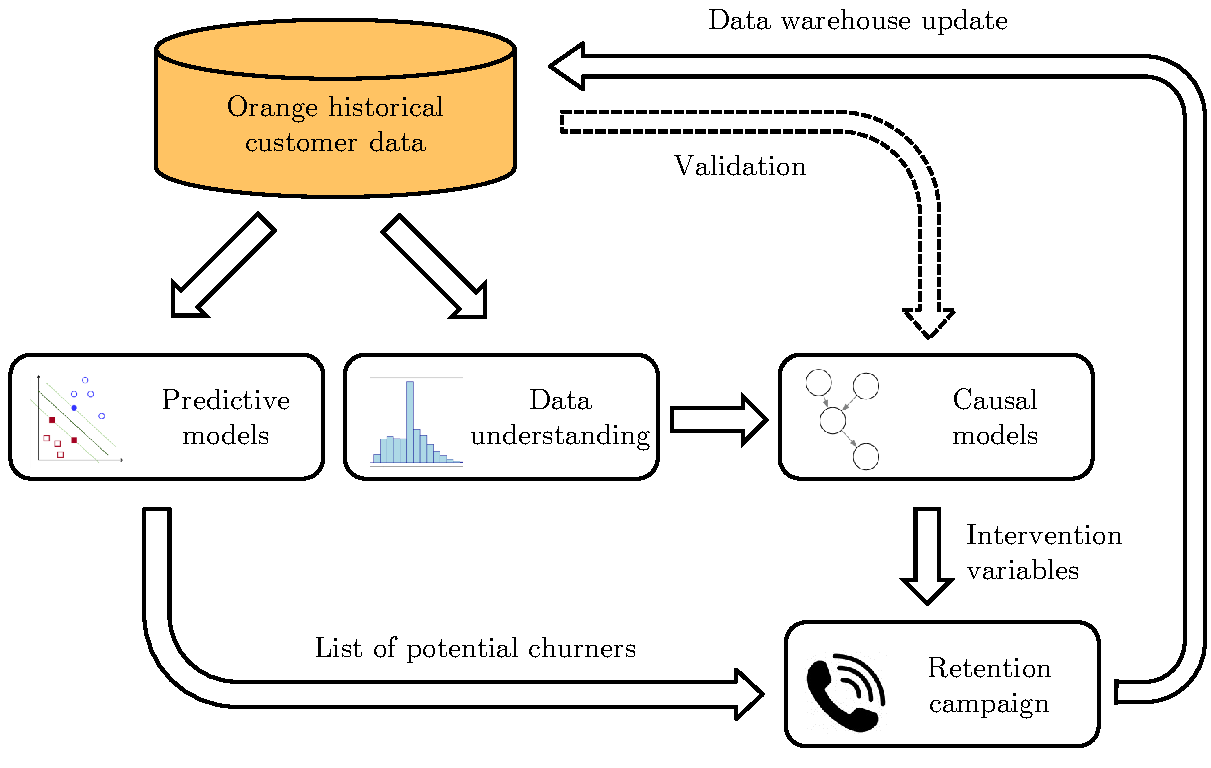
\includegraphics[width=0.95\linewidth]{figures/machu-picchu.pdf}
	\caption{Closed-loop validation process planned for the applied PhD
	project.}
	\label{fig:machu-picchu}
\end{figure}

\subsection{Conclusion}

We approached the churn prediction problem in the telecommunication industry
with Orange Belgium customer data. A descriptive analysis of the dataset has
been conducted, showing the non-linearity of variables, large overlap between
churners and non-churners, non-stationarity and class imbalance. Predictive
modeling of churn was achieved with a random forest classifier and the Easy
Ensemble algorithm. In a series of experiments on churn prediction, we assessed
the impact of variable selection, type of contract and use of engineered
features. The results show that variable selection helps reducing computation
time, but can decrease performance. Also, the addition of features consisting in
the difference and the ratio of numerical variable seems to reduce the
performance. The directionality of the impact of variables on churn is estimated
through a sensitivity analysis. This shows that some variables are associated to
the churn probability in a non-monotonic way. We explored the application of
causal inference from observational data. More specifically, we applied 5
different causal inference methods, namely PC, Grow-Shrink (GS), Incremental
Association Markov Blanket (IAMB), minimum Interaction Maximum Relevance (mRMR),
and D2C. The results of these algorithms are varied, and are partly consistent
with prior knowledge on the causes of churn. This research highlights the
difficulty of carrying out causal inference in a realistic setting, due to the
large variety of variable types and distributions.
